\documentclass{Vorlage}
%\usepackage[ngerman]{babel}
\usepackage{amsfonts}
\usepackage{graphicx}
\usepackage{url}
\usepackage{amsmath}
\usepackage{adjustbox}
\usepackage{color}
\usepackage{multirow}
\usepackage{bm}
%\usepackage[utf8]{inputenc}
%\bibliographystyle{apalike}
\setlength{\parindent}{0pt}

\pagestyle{fancy}
\renewcommand*\sectionmark[1]{\markboth{\MakeUppercase{#1}}{}}
\begin{document}

\newgeometry{top=2.5cm,bottom=2.0cm,left=2.5cm,right=2.5cm} % Befehl wird nur benötigt, falls Änderungen an den Seitenrändern in der Datei "Vorlage.cls" vorgenommen werden.

\begin{titlepage}

\begin{figure}
 \begin{center}
 
\includegraphics[scale=0.8]{Pictures/logo3}
 \end{center}
\end{figure}
\vspace*{3cm}




\titel{Kleinräumige Extrapolation von Umfragedaten}{}

\vspace{1cm}

\begin{tabular}{p{3.5cm}|p{0.1cm} p{10cm}l}
\textsc{Namen:} & & \textsc{Alexander Lange, Kai Husmann}\\
\textsc{Matr. Nr.:} & & \textsc{21426614, 20707176}\\
\textsc{Studiengang:} & & \textsc{Angewandte Statistik}\\
\textsc{Mail:} & & \textsc{Alexander.lange$ @ $uni-goettingen.de}\\
\textsc{} & & \textsc{Kai.Husmann$ @ $forst.uni-goettingen.de}\\
\textsc{Kurs:} & & \textsc{Statistisches Praktikum}\\
\textsc{Kursleiter:} & & \textsc{Prof.Dr. Thomas Kneib}\\
\textsc{Lehrstuhl:} & & \textsc{Statistik}\\
\textsc{Fakultät:} & & \textsc{Wirtschaftswissenschaften}\\
\textsc{Abgabedatum:} & & \textsc{30. September 2016}\\
\end{tabular}
\end{titlepage}

\restoregeometry

\pagenumbering{Roman} % \pagenumbering{roman} = Kleinschreibung: II -> ii.

\pagestyle{plain}

\tableofcontents % Inhaltsverzeichnis.

\newpage % Neue Seite.

\listoffigures % Abbildungsverzeichnis.

\listoftables % Tabellenverzeichnis.

\newpage

\pagenumbering{arabic} % Ab hier folgt die arabische Seitennummerierung.

%\renewcommand{\thesection}{\arabic{section}} % Römische Nummerierung der Kapitelüberschriften.

%============================================ Instroduction ========================================================%
\pagestyle{fancy}

\section{Einleitung}
Die Grundgesamtheit dieser Unteruchung ist die Bevölkerung Stuttgarts.
Fragestellungen: Wie ist die Wohzufriedenheit in Stuttgart? Wie ist die Meinung zu Stuttgart 21? Kleinräumige Extrapolation
test

\newpage

%=================================================== Main Part  ====================================================%
\section{Material und Methoden}
\subsection{Daten}
Insgesamt liegen für die Analysen drei Umfragen mit unterschiedlichen Stichprobenumfängen vor. Die kleinste Datei enthält Angaben zur Bewertung der Wohngegend, der Meinung zu Stutttgart 21 sowie weitere sozioökonomische Kovariablen, die zur Erklärung der beiden abhängigen Variablen dienen sollen. Die Datei wird im Folgenden als Parametrisierungsstichprobe bezeichnet. Bei der Parametrisierungsumfrage handelt es sich folglich um eine Stichprobe von der die Grundgesamtheit für eine Validierung nicht zur Verfügung steht. Alle Modellqualitätskriterien müssen entweder an der Stichprobe selbst oder an den beiden separat erhobenen Umfragen angewendet werden. Diese beiden anderen Umfragen haben jeweils einen deutlich größeren Stichprobenumfang. An diesen Umfragen werden die parametrisierten Modelle angewendet und die Meinung zu Stuttgart 21 sowie die Wohnzufriedenheit somit kleinräumig extrapoliert. Einige Variablen unterscheiden sich in ihren Ausprägungen zwischen den Umfragen. Zur Vereinheitlichung der Dateien mussten einige Gruppenausprägungen demnach umkodiert werden. Die Umkodierungen können in der digital anhängenden Datei \textit{Aufbereitung\_Stuttgart21.R} nachvollzogen werden.

\subsubsection{Parametrisierungsstichprobe}
Mit den Datensätzen der Parametrisierungsstichprobe (Tabelle \ref{Datensatz}) werden die Modelle zur kleinräumigen Extrapolation parametrisiert. Insgesamt beinhaltet die Umfrage 8 sozioökonomische Variablen und Angaben zur räumlichen Lage. Von jedem Datensatz sind die stetige räumliche Lage als Gauss-Krüger Geokoordinate sowie die diskrete räumliche Lage in Stadtteil und Stadtbezirk bekannt.\\

%% Wärst Du einverstanden,wenn wir diese Überschriften rausnehmen? Ich finde, Du hast im Text / in de rTabelle schon sehr deutlich gemacht, dass die Datei hier deskr. beschrieben wird. Gilt dann auch für die rüuml. Effekte. Ich fänds übersichtlicher, wenn wir die 3 Umfrgen als Überschroft nehmen.
%% \subsubsection{Deskriptive Statistik}

\begin{table}[h]
\centering
\caption{Erhobene sozioökonomische und geographische Variablen der Parameterisierungsstichprobe und deren Anzahl der Ausprägungen sowie vermutete Modellierung im additiven Modell.}
\label{Datensatz}
\adjustbox{max height=\dimexpr\textheight-5.5cm\relax,
           max width=\textwidth}{
\begin{tabular}{l|c|c}
\multicolumn{2}{l}{Anzahl Beobachtungen: 3.143}     \\ \hline \hline
\textbf{Variable} & \textbf{Anzahl Ausprägungen} & \textbf{Modellierung} \\ \hline
Bewertung Wohngegend &  6 & Geordnet Kategorial \\ \hline
Meinung Stuttgart 21 &  6 & Geordnet Kategorial \\ \hline
Personenanzahl im Haushalt & 5 & Nicht Parametrisch \\ \hline
Monatliches Netto Haushaltseinkommen & 6 & Nicht Parametrisch \\ \hline
Altersklasse Befragter & 6 & Nicht Parametrisch \\ \hline
Geschlecht & 2 & Parametrisch\\ \hline
Familienstand & 4 & Parametrisch \\ \hline
Nationalität & 2 & Parametrisch \\ \hline
Stadtbezirk & 23 & Markov-Zufallsfeld \\ \hline 
Stadtteil &  142 & Markov-Zufallsfeld \\ \hline 
Gauß-Krüger & & Tensorprodukt-Splines  \\ \hline \hline
\end{tabular}
}
\end{table}


In der Tabelle sind nicht nur die Kategorienanzahlen der Variablen, sondern auch die vermuteten Formen der Einflüsse der Kovariablen auf die abhängigen Variablen aufgelistet. Diese wurden durch visuelle Darstellung aller Kovariablen über den abhängigen Variablen ermittelt. Nach visueller Einschätzung ergab sich, dass alle nominal skalierten Variablen, wie z.B. die Nationalität, als parametrisch und dass alle kardinal skalierte Variablen, wie z.B. die Altersklasse des Befragten, offensichtlich als nicht parametrisch modelliert werden sollten. Diese beobachteten Zusammenhänge finden sich häufig in Regressionsmodellen \cite[p. 9]{fahrmeir2009regression}. In Anlehnung an \cite[p. 503 ff., p. 524 ff.]{fahrmeir2013regression} wird der räumliche Effekt entweder kontinuierlich als Tensor Produkt oder diskret als Gauss-Markov Zufallsfeld modelliert.\\
Für die Auswahl der geeigneten Regressionsmethode ist es hilfreich, das Verhältnis der Häufigkeiten der Kategorienausprägungen der abhängigen Variable zu kennen und seltene Ereignisse zu identifizieren. Während die meisten befragten Personen ihre Wohngegend mit \textit{gut} oder \textit{sehr gut} bewertet haben, treten Beobachtungen mit schlechterer Einschätzung folglich deutlich seltener auf. Zudem sind die Gruppenhäufigkeiten der Antworten zum Projekt Stuttgart 21 näherungsweise gleichverteilt. In beiden Fällen wurden die wenigen, für die Modellierung irrelevanten Kategorien \textit{Keine Angabe} entfernt. In beiden Fällen kann den Gruppen eine Rangfolge, jedoch kein Intervall Abstand unterstellt werden. Es handelt sich demnach jeweils um ordinal Skalierte Daten.

\begin{figure}[h]
 \begin{center}
 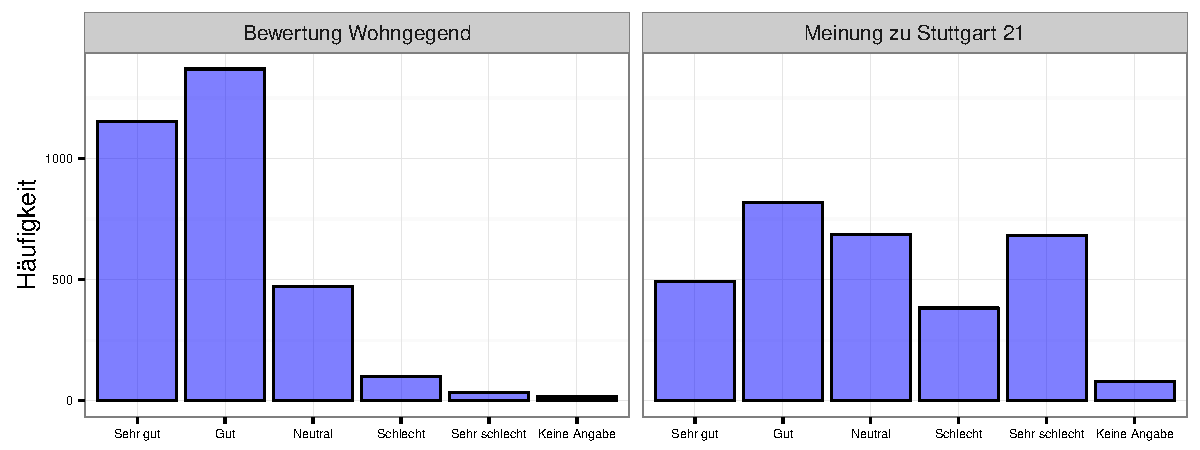
\includegraphics[scale=0.8]{Pictures/BarResp}
 \caption{Endogene Variablen der Parameterisierungsstichprobe.}
 \label{endogene}
 \end{center}
\end{figure}

Das amtliche, nach Stadtteilen oder Stadtbezirken aufgelöste Ergebnis der Volksabstimmung zu Stuttgart 21 von 2011 kann dem Internetauftritt der Stadt entnommen werden \cite{Amt}. Es bietet sich dadurch eine zusätzliche Möglichkeit zur Modellevaluierung an. Da hier mit Sicherheit nur zwei Kategorien (\textit{Zustimmung}, \textit{Ablehnung }) unterschieden werden können, wurden die Daten dieser Arbeit neu gruppiert. Es wurde eine Neugruppierung in drei (\textit{Zustimmung}, \textit{Neutral}, \textit{Ablehnung}, Tabelle \ref{endogene}, links) sowie in zwei Gruppen (\textit{Zustimmung}, \textit{Ablehnung}) vorgenommen. Dafür wurden jeweils die Grppen \textit{sehr gut} und \textit{gut} zu \textit{Zustimmung} und \textit{schlecht} und \textit{sehr schlecht} zu \textit{Ablehnung} zusammengefasst. Außerdem wurden die Beobachtungen mit der Meinung \textit{neutral} für das zwei Klassenmodell entfernt, womit sich hier ein reduzierter Stichprobenumfang von 2377 Beobachtungen ergibt. Dadurch bleibt die Möglichkeit erhalten eine multinomial verlteilte abhängige Variable zu modellieren und trotzdem eine Validierung für zwei Klassen vorzunehmen. Für die exogen in die Analyse einfließenden Variablen sind detailliertere Informationen zu den Häufigkeiten der Ausprägungen im Anhang verfügbar (REF ABB A.1).\\
Da in dieser Arbeit ein Schwerpunkt auf der Analyse unterschiedlicher räumlicher Effekte liegt, vergleicht dieser Abschnitt alle drei räumlichen Effekte in Relation zu den beiden endogenen Variablen. Abbildung \ref{XYStuttgart3} zeigt die absolute Häufigkeit der Beobachtungen der Meinung zu Stuttgart 21 in kontinuierlicher räumlicher Lage. Zur besseren Übersicht wurden nicht alle Beobachtungen geplottet, sondern Beobachtungsdichten über bivariate normalverteilte Kerndichteschätzer mit festem Abstand für jede Richtungen ermittelt \cite{ggplot} sowie \cite{MASS}. Um die Hintergrundkarte einbinden zu können wurden die Gauß-Krüger Koordinaten in Dezimalgrad umgerechnet. Da absolute Dichten dargestellt werden, ist zunächst ersichtlich, in welchen Bereichen die meisten Bürger leben. Wegen der hohen Einwohnerdichte im Innenstadtbereich sind dort die Beobachtungsdichten aller 3 Klassen tendenziell höher als in den Randbezirken. Des weiteren ersichtlich ist, dass einige Bereiche, wie das Naturschutzgebiet \textit{Rotwildpark} im Westen oder der \textit{Schurwald} im Osten, aufgrund ihrer geographischen Beschaffenheit oder Landnutzungsform nicht oder nur sehr dünn besiedelt sind.

\begin{figure}[h]
 \begin{center}
 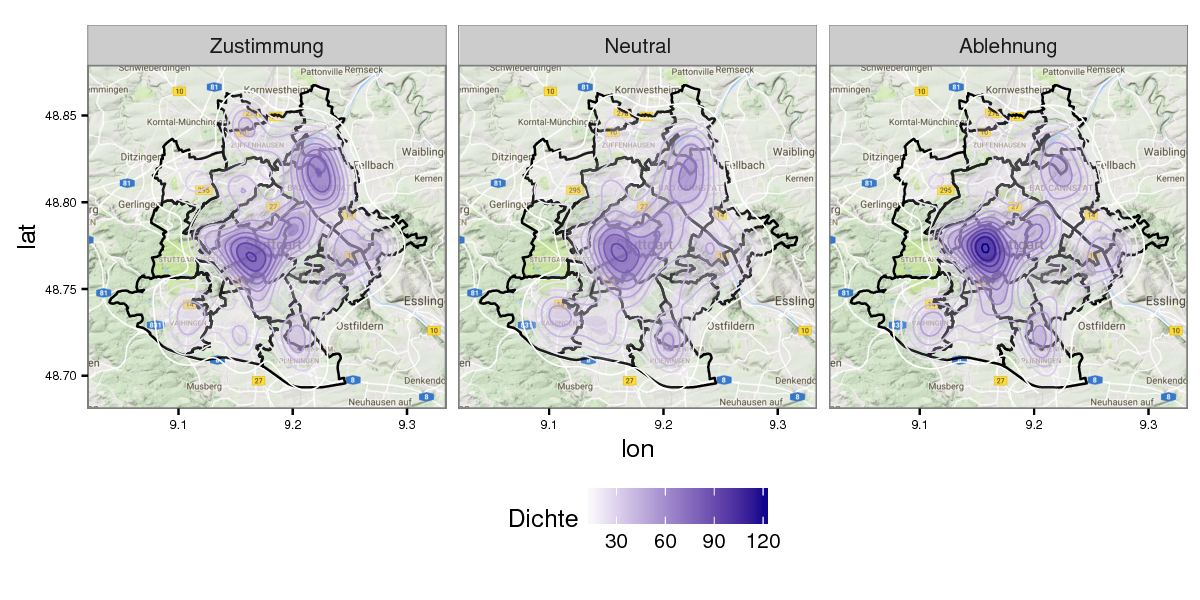
\includegraphics[scale=0.8]{Pictures/XYStuttgart3.png}
 \caption{Kontur Plot der absoluten Anzahl der Gruppenbeobachtungen zur Meinung zu Stuttgart 21 in drei Gruppen. Quelle der Hintergrundgrafik: REF: Google Maps}
 \label{XYStuttgart3}
 \end{center}
\end{figure}

Die \textit{Zustimmung} zeigt offensichtliche räumliche Muster. Im Zentrum und im Nordosten ist sie höher als im Rest der Stadt. Der räumliche Trend der \textit{Ablehnung} ist schwächer ausgeprägt. Es zeigt sich jedoch, dass der Bereich der Innenstadt, sowie die südlichen Stadtbereiche etwas höhere Dichten bei der \textit{Ablehnung} aufweisen. Die Beobachtungen der Kategorie \textit{neutral} sind eher gleichmäßig über die Stadt verteilt.\\
Abbildung \ref{XYWohnG5} zeigt die Dichte der Beobachtungen der fünf Kategorien zur Bewertung der Wohngegend. Hier zeigt sich ein deutlich ausgeprägteres räumliches Muster als bei der Meinung zu Stuttgart 21. Die Beobachtungen der Klasse \textit{sehr gut} häufen sich sehr stark im Innenstadtbereich und im Süden. Die Kategorie \textit{gut} verteilt sich relativ homogen über das gesamte Stadtgebiet mit einer etwas stärkeren Konzentration in der Innenstadt und im Nordosten. Bei der Klasse \textit{neutral} zeigt sich eine stärkere Konzentration auf den Osten und Nordosten der Stadt. Praktisch alle \textit{schlechten} und \textit{sehr schlechten} Bewertungen sind deutlich abgegrenzt im Osten und Nordosten lokalisiert. Hierbei ist zu erwähnen, dass der Anteil der Personen, die ihre Wohngegend mit \textit{schlecht} oder \textit{sehr schlecht} bewertet haben sehr gering ist Abbildung \ref{endogene}.\\

\begin{figure}[h]
 \begin{center}
 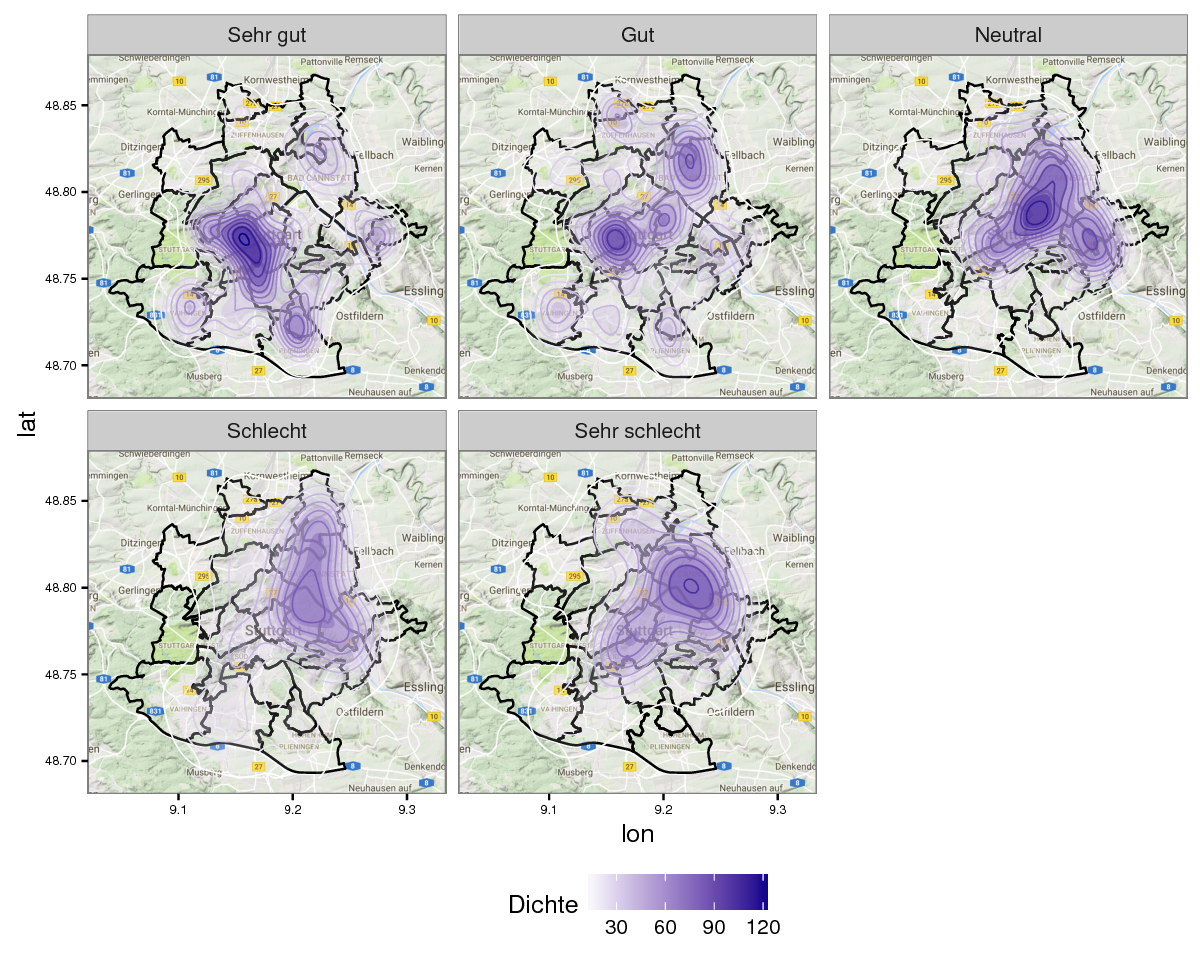
\includegraphics[scale=0.8]{Pictures/XYWohnG5.png}
 \caption{Kontur Plot der absoluten Anzahl der Gruppenbeobachtungen zur Wohnzufriedenheit in fünf Gruppen. Quelle der Hintergrundgrafik: REF: Google Maps}
 \label{XYWohnG5}
 \end{center}
\end{figure}


Im folgenden werden die diskreten räumlichen Informationen auf Stadtbezirksebene beschrieben. Es werden 23 Stadtbezirke 
unterschieden. Im Gegensatz zur stetigen Beobachtungsdichte werden die Beobachtungen nach Regionen aggregiert 
dargestellt, wodurch eine relative Anteilsdarstellung möglich wird (Abbildung \ref{BStuttgart21}). Die Darstellung wird 
also weniger von der absoluten Gesamtbevölkerungsdichte in den Regionen überdeckt. Analog zur stetigen Darstellung 
(Abbildung \ref{XYStuttgart3}) ist auch hier zu sehen, dass die Bürger des Nordostens eine positivere Meinung zu 
Stuttgart 21 haben als die Bürger aus dem Süden. Die neutrale Klasse hat in allen Bezirken einen geringeren Anteil und es ist kein räumliches Muster erkennbar. Die entsprechenden Anteilsgrafiken mit fünf Klassen für die Bewertung der Wohngegend sind im Anhang verfügbar (Abbildung 
\ref{BWohn}). Wie in Abbildung \ref{XYWohnG5} bereits angedeutet, zeigen sich negative Wohngebietseinschätzungen vor 
allem im Nordosten.

\begin{figure}[h]
 \begin{center}
 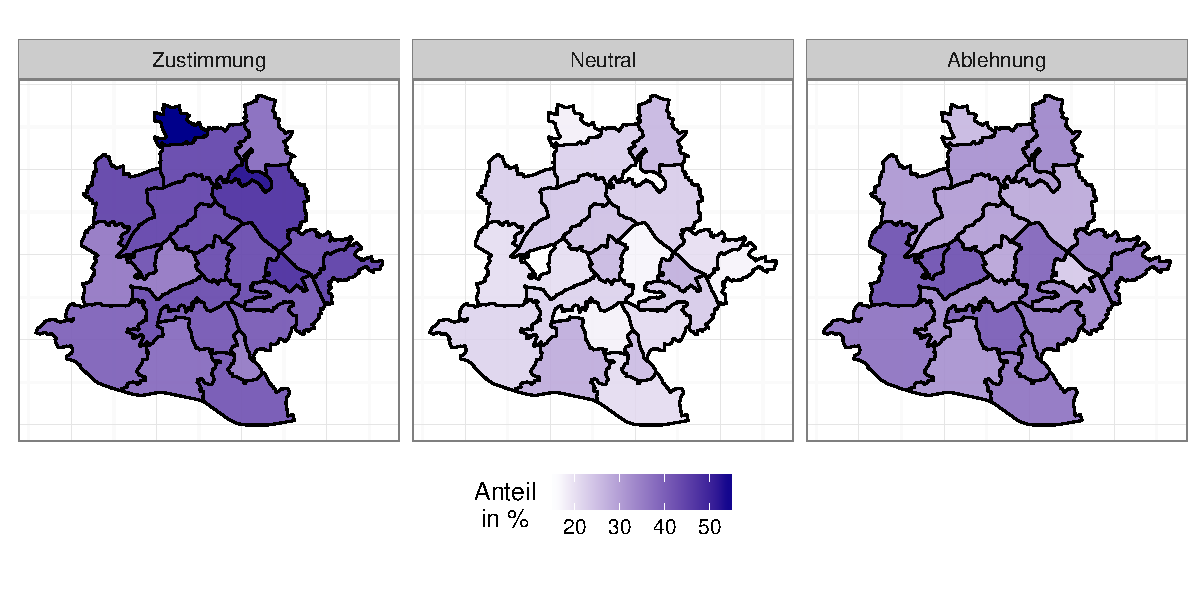
\includegraphics[scale=0.8]{Pictures/BStuttgart3}
 \caption{Anteile zur Meinung zu Stuttgart 21 nach Stadtbezirken.}
 \label{BStuttgart21}
 \end{center}
\end{figure}

Die dritte und letzte untersuchte räumliche Agrregationsebene ist die Stadtteilebene. Abbildung \ref{SStuttgart21} 
zeigt die räumliche Verteilung von \textit{Zustimmung}, \textit{Ablehnung} und \textit{neutraler} Haltung. Wie aus 
Tabelle \ref{Datensatz} hervorgeht, ist die Stadtteilebene deutlich feiner Aufgelöst als die Bezirksebene. Dies führt in 
der Abbildung dazu, dass einige Stadtteile mit geringer Gesamteinwohneranzahl in einer oder mehreren Klassen keine 
Beobachtungen zeigen. Es gibt demnach auch Stadtteile, in denen die komplementäre Klasse zu 100 \% vertreten ist. Des 
weiteren gibt es in dieser Aggregationsebene sogar Stadtteile ohne jede Beobachtung, wie z. B. das Benzviertel im 
Innenstadtbereich oder die bereits angesprochenen Lagen im Westen.

\begin{figure}[h]
 \begin{center}
 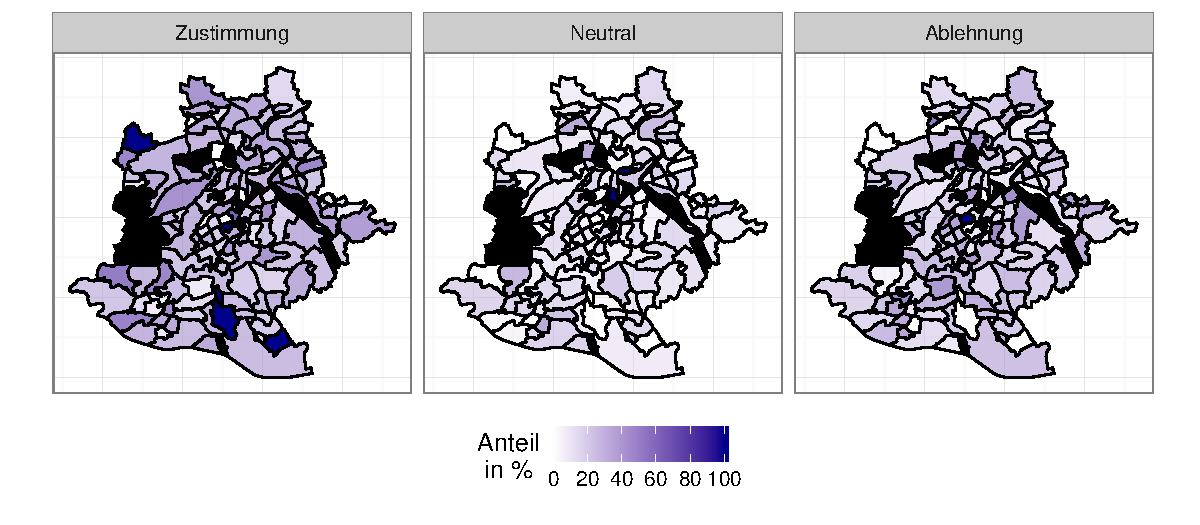
\includegraphics[scale=0.8]{Pictures/SStuttgart3}
 \caption{Anteile der Meinung zu Stuttgart 21 nach Stadtteilen.}
 \label{SStuttgart21}
 \end{center}
\end{figure}

Diese Stadtteile werden in den Diagrammen schwarz dargestellt. Wegen der feineren Auflösung ergibt sich ein mosaikartiges, visuell schwerer interpretierbares Bild. In keiner der drei Klassen lässt sich eine klare Struktur oder räumliches Muster erkennen. Die Anteile auf Stadtteileebene zu der Bewertung der Wohngegend sind im Anhang verfügbar \ref{SWohn}. Hier zeigt sich ein ähnlich schwer differenzierbares Muster wie bei der Meinung zu Stuttgart 21. Wegen der deutlichen Unterschiede in den Anteilen der fünf Gruppen sind die Farbskalen nicht einheitlich, sondern unterscheiden sich in den Diagrammen.\\

\subsubsection{Bürgerumfrage}
In der Bürgerumfrage von 20?? wurden 470.190 Bürger zu acht sozioökonomischen Punkten befragt. Der Stichprobenumfang dieser Umfrage liegt also relativ nah an der Grundgesamtheit von 573.104 Bürgern, die 2011 mit Hauptwohnsitz in Stuttgart gemeldet waren (REF Stat. Bundessamt). Von allen Befragten liegt der Wohnsitz als kontinuierliche Gauss-Krüger Geokoordinate vor. Um eine kleinräumige Extrapolation mit diskreten räumlichen Informationen vornehmen zu können, wurden die Stadtteil- und Stadtbezirksinformationen an die Datei angehängt. Hierzu wurden die Stadtteil- und Stadtbezirkspolygone, welche uns von der Stadt Stuttgart zur Verfügung gestellt wurden, über eine räumliche Abfrage mit der Bürgerumfrage Datei verknüpft. Die Geoanalyse wurde mit dem freien Geoinformationssystem QGIS (REF) durchgeführt. Die Projektdatei mit der Geoabfrage (\textit{Geographische\_Abfrage.QGS}) sowie die Shapefiledateien (\textit{Stadtteile\_netto.SHP}) liegen dieser Arbeit digital bei. Wie in den Tabellen \ref{Datensatz} und REF ? ersichtlich eignen sich nicht alle Variablen zur Extrapolation, da nicht alle Variablen in jeder Umfrage erhoben wurden. Es ergibt sich ein Überschneidungsbereich der fünf sozioökonomischen Variablen \textit{Altersklasse Befragter}, \textit{Geschlecht}, \textit{Nationalität}, \textit{Familienstand} und \textit{Personenzahl im Haushalt}. \textcolor{red}{IN TAB 2 BRAUCHEN WIR DIE SPALTE MODLLEIRUNG EIGENTLICH NICHT MEHR ODER? ICH HABE DIE VARIABLEN Z.T. UMBEBENANNT, DAMIT SIE GLEICH HEIßen WIE IN TAB 1. AUßERDEM SIND JA NACH DEM UMKODIEREN BEI DER ALTERSKLASSE NUR NOCH  6 AUSPR. ICH WÜRDE DAS IN DER TAB. 2 ANPASSEN WAS MEINST DU?}

\begin{table}[h]
\centering
\caption{Erhobene sozioökonomische und geographische Variablen der Bürgerumfrage und deren Anzahl der Ausprägungen.}
\adjustbox{max height=\dimexpr\textheight-5.5cm\relax,
           max width=\textwidth}{
\begin{tabular}{l|c|c}
\multicolumn{3}{l}{Anzahl Beobachtungen: 470.190}     \\ 
\hline \hline
\textbf{Variable} & \textbf{Modellierung} & \textbf{Anzahl Ausprägungen}  \\ \hline
\multicolumn{1}{l|}{Altersklasse Befragter} &  Nicht Parametrisch & 14 \\ \hline
\multicolumn{1}{l|}{Geschlecht} &  Parametrisch  & 2 \\ \hline
\multicolumn{1}{l|}{Nationalität} & Parametrisch  & 2 \\ \hline
\multicolumn{1}{l|}{Familienstand} & Parametrisch & 4 \\ \hline
\multicolumn{1}{l|}{Personenzahl im Haushalt} &  Nicht Parametrisch  & 5 \\ \hline
\multicolumn{1}{l|}{Wohndauer} & Nicht Parametrisch  & 3 \\ \hline
\multicolumn{1}{l|}{ALG II Quote} & Nicht Parametrisch  & 9 \\ \hline
\multicolumn{1}{l|}{Ein/Zweifamilienhäuser}& Nicht Parametrisch & 8 \\ \hline 
\multicolumn{1}{l|}{Gauß-Krüger} & Tensorprodukt-Splines & \\ \hline \hline
\end{tabular}

}
\end{table}

\subsubsection{Zensus}
Im Rahmen der bundeweiten Volkszählung von 2011 wurden in Stuttgart 380.238 Bürger befragt \textcolor{red}{REF TAB 3}. Da beim Zensus auch für die Fragestellung dieser Arbeit relevante sozioökonomische Variablen erhoben wurden, eignet sich diese Umfrage ebenfalls für die kleinräumige Extrapolation. Die diskreten geographischen Angaben wurden analog zur Bürgerumfrage per geographischer Abfrage ergänzt. Für die kleinräumige Extrapolation eignen sich die gleichen möglichen sozioökonomischen Variablen wie bei der Bürgerumfrage. 
\textcolor{red}{Wie in Tab. 2.: Habe die Namen angepasst. Anzahl Personenzahl und Alter umkodiert, also auch in Tabelle ändern? Wir könnten sogar überlegen, die nicht verwendeten Variablen zu löschen. Wir gehen ja im Text nicht mehr auf diese ein (gilt auch für Tab 2)}

\begin{table}[h]
\centering
\caption{Erhobene sozioökonomische und geographische Variablen der Bürgerumfrage und deren Anzahl der Ausprägungen.}
\adjustbox{max height=\dimexpr\textheight-5.5cm\relax,
           max width=\textwidth}{
\begin{tabular}{l|c|c}
\multicolumn{3}{l}{Anzahl Beobachtungen: 380.238}     \\ 
\hline \hline
\textbf{Variable} & \textbf{Modellierung} & \textbf{Mögliche Ausprägungen}  \\ \hline
\multicolumn{1}{l|}{Altersklasse Befragter} &  Nicht Parametrisch & 9 \\ \hline
\multicolumn{1}{l|}{Geschlecht} & Parametrisch  & 2 \\ \hline
\multicolumn{1}{l|}{Nationalität} & Parametrisch  & 2 \\ \hline
\multicolumn{1}{l|}{Familienstand} & Parametrisch & 4 \\ \hline
\multicolumn{1}{l|}{Personenzahl im Hasuhalt} &  Nicht Parametrisch  & 6 \\ \hline
\multicolumn{1}{l|}{Wohnfläche} & Nicht Parametrisch & 24 \\ \hline
\multicolumn{1}{l|}{Stellung Beruf} & Parametrisch  & 9 \\ \hline
\multicolumn{1}{l|}{Beamter}& Parametrisch & 2 \\ \hline 
\multicolumn{1}{l|}{Gebäudetyp}& Parametrisch & 10 \\ \hline
\multicolumn{1}{l|}{Gebäudenutzung}& Parametrisch & 2 \\ \hline
\multicolumn{1}{l|}{Gauß-Krüger} & Tensorprodukt-Splines & \\ \hline \hline
\end{tabular}

}
\end{table}


\subsection{Statistische Methoden}

\subsubsection{Modell}
Kurze Erläuterung GAM und logit,... Zusammengesetzt aus parametrischen Effekten und Splines. Pseudobeobachtungen. Wahl 
des Glättungsparameters  (Wood 2000).

\subsubsection{Modellwahl}
Basierend auf den vorhergegangenen Analysen des Beamten- und Eigenheimanteils in Stuttgart wurde die R Funktion 
\texttt{stepAIC()} zur schrittweisen AIC \cite{Akaike1981} Berechnung programmiert, die zur Identifikation der 
geeignetsten Kovariablenkombination dient. In der Funktion werden mithilfe der \texttt{gam()} Funktion des \texttt{mgcv} 
Paketes \cite{Wood2011} generaliserte additive Modelle mit unterschiedlichen Kovariablen erstellt und deren AIC 
berechnet. Vor dem Aufruf der Funktion müssen die abhängige Variable, die Verteilungsannahme des Regressionsmodelles, 
die Gewichtungen der Einzelbeobachtungen und unveränderliche Kovariablen definiert werden. Außerdem muss eingeschätzt 
werden, welche der veränderlichen Kovariablen parametrisch oder semiparametrisch als Spline in das Modell eingehen. Es 
wird zunächst der AIC des einfachsten, nur aus den fest vorgegebenen Kovariablen bestehenden Modells berechnet. In 
Iteration eins werden alle veränderlichen Kovariablen einzeln nacheinander in die Modellformel aufgenommen und es wird 
jeweils ein GAM erstellt sowie dessen AIC berechnet. Die Kovariablen gehen entsprechend der vorigen Eingabe parametrisch 
oder semiparametrisch ein. Falls die Hinzunahme mindestens einer Kovariable in Iteration eins zu einer Reduktion des AIC 
führt, wird diejenige Kovariable, welche zu dem Modell mit dem kleinsten AIC führt zur Modellformel hinzugefügt. Falls 
das Modell nur mit den festen Modellbestandteilen bereits den geringsten AIC zeigt ist die Modellwahl folglich in 
Iteration eins bereits beendet.\\ Andernfalls setzt sich das Ausgangsmodell für Iteration zwei aus den festen 
Kovariablen und einer weiteren Kovariable zusammen. In Iteration zwei werden wie zuvor alle verbleibenden Kovariablen 
zunächst nacheinander zur aktuellen Modellformel hinzugefügt. Wenn die Kovariable mit dem geringsten AIC gefunden ist 
(falls diese existiert und das Modell aus Iteration eins nicht bereits das geeignetste ist), werden alle veränderbaren 
Kovariablen in Iteration zwei nochmals nacheinander eliminiert. Das Modell mit dem geringsten AIC bildet das 
Ausgangsmodell der nächsten Iteration. Dies wird wiederholt bis in einer Iteration kein Modell mit einem geringeren AIC 
als in der vorigen Iteration parametrisiert werden kann. Um die Laufzeit der Funktion zu begrenzen, wurde auf die 
Analyse von Wechselwirkungen zwischen den Kovariablen verzichtet. Wechselwirkungen können jedoch als unveränderliche 
Modellbestandteile eingehen.

\subsubsection{Konfidenzbänder}
Die Intervalle der Punktschätzungen liefern zusätzliche wichtige Informationen, da die Punktschätzungen alleine keine 
Angaben zur Unsicherheit enthalten. Mit dem Vertrauensintervall erhält man die Relation der Unsicherheit zur 
Punktschätzung zur Unsicherheit und somit ein weiteres Modellgütemerkmal \cite[p. 471]{fahrmeir2013regression}. Des 
weiteren eignen sich Konfidenzintervalle zur Formulierung von Hypothesentests und zur Berechnung von 
Überdeckungswahrscheinlichkeiten bestimmter Werte von Interesse. Grundsätzlich gibt es die Möglichkeit intervalle aus 
den Modellinformationen abzuleiten oder Bootstrap-Intervalle durch wierderholte zufällige Reparametrisierung 
des Modells zu berechnen. Bei ersterem Vorgehen sind, je nach Methode, oft zusätzliche Annahmen, beispielsweise zur 
Verteilung oder zur Symmetrie, der Intervalle zu treffen. Aus diesen Gründen wurden punktweise Bootstrap-Intervalle für 
jede Punktschätzung berechnet.\\
Zur Berechnung der Intervalle wurde jedes Modell 1.000 mal mit einer Zufallsstichprobe (\textit{Ziehen-mit-Zurücklegen}) 
aus der Parameterisierungsstichprobe prametrisiert. Um den Einfluss des Stichprobenumfangs zu eliminieren, enthielt 
jede Stichprobe die tatsächliche Anzahl der Beobachtungen. Aus den Wiederholungen wurden arithmetischer Mittelwert, 
Median, unteres sowie oberes 95 \% Perzentil berechnet.



\subsubsection{Kreuzvalidierung}
Für die Modellerstellung der additiven Modelle lag eine Stichprobe von 3.143 vor. Außer der Gesamtindividuenanzahl 
(573.104 gemeldete Bürger) lagen keine Informationen zur Grundgesamtheit vor. Die Qualität der Modelle ließ sich 
folglich nicht an der Grundgesamtheit validieren sondern musste an der Stichprobe selbst eingeschätzt werden. Zu diesem 
Zweck wurde eine \textit{Leave-One-Out} Kreuzvalidierung durchgeführt \cite[p. 149]{fahrmeir2013regression}, in welcher 
jeweils eine beobachtung zufällig entfernt wurde. Die verbleibenden Beobachtungen wurden genutzt, um ein additives 
Moell zu erstellen, mit dem die entfernte Beobachtung vorhergesagt wurde. Mit diesen Daten ließ sich ein Statistik zu 
den korrekt reklassifizierten Beobachtungen erstellen.


\subsubsection{Validierung}
Ziel der Validierung ist es, die prognostizierten Anteile aus dem gewählten Modell mit den wahren Anteilen aus der 
Volksabstimmung \cite{Amt} zu vergleichen, um eine Aussage über die Qualität der geschätzten Prognosemodelle geben zu 
können. Die Validierung erfolgt auf Stadtteil- und Bezirksebene, sowie für das Gesamtergebnis der Stadt Stuttgart. Dazu 
werden insbesondere zwei statistische Gütemaße verwendet.\\
Bei der Wahl des Schätzers geht es zum einen darum, einen möglichst erwartungstreuen als auch effizienten Schätzer zu 
finden. Als geeignetes Gütemaß hat sich die mittlere quadratische Abweichung erwiesen, da sie sowohl die Varianz, als 
auch die quadrierte Verzerrung berücksichtigt. Zudem hat ein konsistenter Schätzer die Eigenschaft, dass die mittlere 
quadratische Abweichung bei unendlich groß werdender Stichprobe gen Null konvergiert \cite[p. 201]{HOG}. Ein weiteres 
Kriterium ist die Überdeckungswahrscheinlichkeit. Sie gibt an, mit welcher Wahrscheinlichkeit das geschätzte 
Konfidenzintervall den wahren Wert enthält. Erwartet wird hier, dass die Überdeckungswahrscheinlichkeit dem 
Konfidenzniveau entspricht. Mögliche größere Abweichungen können durch die Approximation einer diskreten Verteilung 
durch eine stetige Verteilung resultieren, was z.B. oft bei der Approximation der Binomial- durch die Normalverteilung 
vorkommt \cite[p. 102]{Int}.

\section{Ergebnisse}

\subsection{Modellwahl}

\subsection{Modell}

\subsection{Reklassifizierung}

Die Ergebnisse der Reklassifizierung zur Meinung zu Stuttgart 21 (Tabelle \ref{evalS21}) zeigen, dass die Erfolgsquote im drei Klassenmodell zwischen 44\% und 50\% liegt und im zwei Klassenmodell zwischen 55\% und 62\% liegt. Zum Vergleich mit einem reinen Zufallsmodell, dass im drei Klassenmodell eine Erfolgswahrscheinlichkeit von 1/3 und im zwei Klassenmodell von 1/2 hat, weißen die geschätzten Modelle eine höhere Erfolgsquote auf. Auch bei einem Vergleich mit Tabelle \ref{endogene} zeigt sich, dass die geschätzten Modelle besser abschneiden, als ein triviales Wählen der immer gleichen Klasse.

\begin{table}[h]
\centering
\caption{Reklassifizierung der Meinung zu Stuttgart 21}
\label{evalS21}
\begin{tabular}{ll|c|c|c}
\hline \hline
                          &              & \multirow{2}{*}{Geoadditives Modell} & Modell ohne       & Modell nur mit    \\
                          &              &                                      & räumlichem Effekt & räumlichem Effekt \\ \hline
\multirow{3}{*}{Drei Kl.} & Gauss-Krüger & 0,4918                               & 0,4716            & 0,4732            \\
                          & Bezirke      & 0,4726                               & 0,4719            & 0,4726            \\
                          & Stadtteile   & 0,451                                & 0,4685            & 0,4449            \\ \hline
\multirow{3}{*}{Zwei Kl.} & Gauss-Krüger & 0,6193                               & 0,6104            & 0,5524            \\
                          & Bezirke      & 0,6079                               & 0,6104            & 0,5515            \\
                          & Stadtteile   & 0,6282                               & 0,6052            & 0,6099            \\ \hline \hline
\end{tabular}
\end{table}

Des weiteren ist zu sehen, dass das Geoadditive Modell in fast allen Fällen die höchste Erfolgsquote aufweist. Abweichungen bestehen im drei Klassenmodell mit Stadtteilen als räumlichem Effekt und im zwei Klassenmodell mit Bezirken als räumlichem Effekt. Außerdem ist zu beachten, dass im drei Klassenmodell das Modell nur mit räumlichem Effekt besser abschneidet als das Modell ohne räumlichem Effekt, während sich für zwei Klassen diese Situation umgekehrt hat.\\
Für die Reklassifikation der Bewertung der Wohngegend (Tabelle \ref{evalB}) ergibt sich eine Erfolgsquote zwischen 40\% und 50\%. Damit ist auch hier eine deutliche Verbesserung gegenüber reinem Raten oder dauerhaftem wählen einer Klasse gegeben. 

\begin{table}[h]
\centering
\caption{Reklassifizierung der Bewertung der Wohngegend}
\label{evalB}
\begin{tabular}{l|c|c|c}
\hline \hline
             & \multirow{2}{*}{Geoadditives Modell} & Modell ohne       & Modell nur mit    \\
             &                                      & räumlichem Effekt & räumlichem Effekt \\ \hline
Gauss-Krüger & 0,4922                               & 0,4461            & 0,4896            \\
Bezirke      & 0,4701                               & 0,4461            & 0,4621            \\
Stadtteile   & 0,4046                               & 0,4204            & 0,4347            \\ \hline \hline
\end{tabular}
\end{table}

Für die Modelle mit den kontinuierlichen Gauss-Krüger Informationen und den Bezirken als räumlichem Effekt hat das Geoadditive Modell die höchste Erfolgsrate, wohingegen für die Stadtteilinformationen das Modell nur mit räumlichem Effekt die beste Reklassifizierung aufweist. Insgesamt schneidet das Geoadditive Modell für beide endogene Variablen und alle drei möglichen Klassenanzahlen am besten ab. Außer bei dem zwei Klassenmodell zur Meinung zu Stuttgart 21 weisen beim Geoadditivem Modell die Gauss-Krüger Informationen als räumliche Effekte die höchste und die Stadtteile als räumliche Effekte die niedrigste Erfolgsrate auf. Da die Modelle ohne- oder nur mit räumlichem Effekt in der AIC-Untersuchung und Reklassifizierung in den meisten Fällen schlechter Abschnitten, wurden die Ansätze ohne- oder nur mit räumlichem Effekte nicht weiter verfolgt.

\subsection{Kreuzvalidierung}

% Please add the following required packages to your document preamble:
% \usepackage{multirow}
\begin{table}[h]
\centering
\caption{Kreuzvalidierung der Meinung zu Stuttgart 21 nach einzelnen Klassen}
\label{KreuzM}
\begin{tabular}{lcccccccccc}
\hline
\multicolumn{11}{c}{Drei Klassen}                                                                                                                                                                                                        \\ \hline
\multicolumn{1}{c}{}                                                     & \multicolumn{1}{c|}{}  & \multicolumn{3}{c|}{Gauss-Krüger}            & \multicolumn{3}{c|}{Bezirke}                 & \multicolumn{3}{c}{Stadtteile}         \\ \cline{3-11} 
                                                                         & \multicolumn{1}{c|}{}  & \multicolumn{9}{c}{Geschätzte Klasse}                                                                                                \\
                                                                         & \multicolumn{1}{c|}{}  & 1       & 2   & \multicolumn{1}{c|}{3}       & 1       & 2   & \multicolumn{1}{c|}{3}       & 1           & 2           & 3          \\ \hline
\multirow{3}{*}{\begin{tabular}[c]{@{}l@{}}Wahre \\ Klasse \end{tabular}} & \multicolumn{1}{c|}{1} & 0,756   & 0   & \multicolumn{1}{c|}{0,244}   & 0,754   & 0   & \multicolumn{1}{c|}{0,246}   & +           & +           & +          \\
                                                                         & \multicolumn{1}{c|}{2} & 0,673   & 0   & \multicolumn{1}{c|}{0,327}   & 0,670   & 0   & \multicolumn{1}{c|}{0,330}   & +           & +           & +          \\
                                                                         & \multicolumn{1}{c|}{3} & 0,521   & 0   & \multicolumn{1}{c|}{0,479}   & 0,511   & 0   & \multicolumn{1}{c|}{0,489}   & +           & +           & +          \\ \hline
\multicolumn{2}{l|}{Klassifikation Modell}                                                        & \multicolumn{3}{c|}{\multirow{2}{*}{0,4905}} & \multicolumn{3}{c|}{\multirow{2}{*}{0,4928}} & \multicolumn{3}{c}{\multirow{2}{*}{+}} \\
\multicolumn{2}{l|}{Insgeasmt}                                                                    & \multicolumn{3}{c|}{}                        & \multicolumn{3}{c|}{}                        & \multicolumn{3}{c}{}                   \\ \hline
\multicolumn{11}{c}{Zwei Klassen}                                                                                                                                                                                                        \\ \hline
                                                                         & \multicolumn{1}{l|}{}  & \multicolumn{3}{c}{Gauss-Krüger}             & \multicolumn{3}{c}{Bezirke}                  & \multicolumn{3}{c}{Stadtteile}         \\ \cline{3-11} 
                                                                         & \multicolumn{1}{l|}{}  & \multicolumn{9}{c}{Geschätzte Klasse}                                                                                                \\
                                                                         & \multicolumn{1}{l|}{}  & 1       & \multicolumn{2}{c|}{2}             & 1       & \multicolumn{2}{c|}{2}             & 1           & \multicolumn{2}{c}{2}    \\ \hline
Wahre                                                                    & \multicolumn{1}{l|}{1} & 0,747   & \multicolumn{2}{c|}{0,253}         & 0,732   & \multicolumn{2}{c|}{0,268}         & +           & \multicolumn{2}{c}{+}    \\
Klasse                                                                   & \multicolumn{1}{l|}{2} & 0,538   & \multicolumn{2}{c|}{0,462}         & 0,545   & \multicolumn{2}{c|}{0,455}         & +           & \multicolumn{2}{c}{+}    \\ \hline
\multicolumn{2}{l|}{Klassifikation Modell}                                                        & \multicolumn{3}{c|}{\multirow{2}{*}{0,6193}} & \multicolumn{3}{c|}{\multirow{2}{*}{0,6079}} & \multicolumn{3}{c}{\multirow{2}{*}{+}} \\
\multicolumn{2}{l|}{Insgesamt}                                                                    & \multicolumn{3}{c|}{}                        & \multicolumn{3}{c|}{}                        & \multicolumn{3}{c}{}                   \\ \hline
\end{tabular}
\end{table}

% Please add the following required packages to your document preamble:
% \usepackage{multirow}
\begin{table}[h]
\centering
\caption{Kreuzvalidierung der Bewertung der Wohngegend nach einzelnen Klassen}
\label{KreuzBew}
\begin{tabular}{lc|ccccccccccccccc}
\hline \hline
\multicolumn{1}{c}{}                                                     &   & \multicolumn{5}{c|}{Gauss-Krüger}              & \multicolumn{5}{c|}{Bezirke}                   & \multicolumn{5}{c}{Stadtteile}              \\ \cline{3-17} 
                                                                         &   & \multicolumn{15}{c}{Geschätzte Klasse}                                                                                                        \\
                                                                         &   & 1     & 2     & 3 & 4 & \multicolumn{1}{c|}{5} & 1     & 2     & 3 & 4 & \multicolumn{1}{c|}{5} & 1       & 2       & 3       & 4   & 5       \\ \hline
\multirow{5}{*}{\begin{tabular}[c]{@{}l@{}}Wahre \\ Klasse\end{tabular}} & 1 & 0,445 & 0,555 & 0 & 0 & \multicolumn{1}{c|}{0} & 0,387 & 0,613 & 0 & 0 & \multicolumn{1}{c|}{0} & 0,495   & 0,478   & 0,019   & 0   & 0,008   \\
                                                                         & 2 & 0,254 & 0,746 & 0 & 0 & \multicolumn{1}{c|}{0} & 0,252 & 0,748 & 0 & 0 & \multicolumn{1}{c|}{0} & 0,300   & 0,671   & 0,023   & 0   & 0,006   \\
                                                                         & 3 & 0,149 & 0,845 & 0 & 0 & \multicolumn{1}{c|}{0} & 0,153 & 0,847 & 0 & 0 & \multicolumn{1}{c|}{0} & 0,142   & 0,771   & 0,079   & 0   & 0,008   \\
                                                                         & 4 & 0,141 & 0,859 & 0 & 0 & \multicolumn{1}{c|}{0} & 0,141 & 0,859 & 0 & 0 & \multicolumn{1}{c|}{0} & 0,099   & 0,474   & 0,349   & 0   & 0,078   \\
                                                                         & 5 & 0,114 & 0,886 & 0 & 0 & \multicolumn{1}{c|}{0} & 0,086 & 0,914 & 0 & 0 & \multicolumn{1}{c|}{0} & 0,031   & 0,275   & 0,556   & 0   & 0,138   \\ \hline
\multicolumn{2}{l|}{Klassifik.}                                              & \multicolumn{5}{c|}{\multirow{3}{*}{0.4918}}   & \multicolumn{5}{c|}{\multirow{3}{*}{0,4704}}   & \multicolumn{5}{c}{\multirow{3}{*}{0,4594}} \\
\multicolumn{2}{l|}{Modell}                                                  & \multicolumn{5}{c|}{}                          & \multicolumn{5}{c|}{}                          & \multicolumn{5}{c}{}                        \\
\multicolumn{2}{l|}{Insgesamt}                                               & \multicolumn{5}{c|}{}                          & \multicolumn{5}{c|}{}                          & \multicolumn{5}{c}{}                        \\ \hline  \hline
\end{tabular}
\end{table}

\subsection{Validierung}
% Please add the following required packages to your document preamble:
% \usepackage{multirow}
\begin{table}[h]
\centering
\caption{Vergleich der mittleren quadratischen Abweichung (MSE) und der Überdeckungswahrscheinlichkeit bei allen Prognosen aus den geschätzten Modellen und den beiden Extrapolationsdateien für die Meinung zu Stuttgart 21}
\label{vali}
\begin{tabular}{llll|cc|cc}
\hline \hline
                        &                               &                          &   & \multicolumn{2}{c|}{MSE} & \multicolumn{2}{c}{Überdeckungswk.} \\
                        &                               &                          &   & Zustimmung  & Ablehnung  & Zustimmung        & Ablehnung       \\ \hline
\multirow{12}{*}{3 Kl.} & \multirow{4}{*}{Gauss-Krüger} & \multirow{2}{*}{Bez.}    & U & 0,04        & 0,749      & 1                 & 0,043           \\
                        &                               &                          & Z & 0,116       & 0,557      & 0,391             & 0               \\ \cline{3-8} 
                        &                               & \multirow{2}{*}{Sadtt.}  & U & 0,461       & 5,708      & 0,954             & 0,139           \\
                        &                               &                          & Z & 0,813       & 4,415      & 0,553             & 0,02            \\ \cline{2-8} 
                        & \multirow{4}{*}{Bezirke}      & \multirow{2}{*}{Bez.}    & U & 0,041       & 0,756      & 1                 & 0,043           \\
                        &                               &                          & Z & 0,117       & 0,562      & 0,522             & 0               \\ \cline{3-8} 
                        &                               & \multirow{2}{*}{Stadtt.} & U & 0,482       & 5,678      & 0,934             & 0,139           \\
                        &                               &                          & Z & 0,835       & 4,38       & 0,567             & 0,027           \\ \cline{2-8} 
                        & \multirow{4}{*}{Stadtteile}   & \multirow{2}{*}{Bez.}    & U & 0,032      & 0,862     &      1             &   0,043          \\
                        &                               &                          & Z & 0,148       & 0,552      &     0,478         &     0 \\ \cline{3-8} 
                        &                               & \multirow{2}{*}{Stadtt.} & U & 0,646       & 6,367       &   0,947           &   0,225  \\
                        &                               &                          & Z & 1,078        & 4,336       &   0,66           &                0,1 \\ \hline
\multirow{12}{*}{2 Kl.}  & \multirow{4}{*}{Gauss-Krüger} & \multirow{2}{*}{Bez.}   & U & 0,312      & 0,312      &     0,826           &  0,826
 \\
                        &                               &                          & Z & 0,152      & 0,152      &   0,522           &  0,522     \\ \cline{3-8} 
                        &                               & \multirow{2}{*}{Stadtt.} & U & 2,694       & 2,679     &   0,649          &  0,649   \\
                        &                               &                          & Z & 1,581       & 1,569      &  0,46            &   0,46   \\ \cline{2-8} 
                        & \multirow{4}{*}{Bezirke}      & \multirow{2}{*}{Bez.}    & U & 0,312       & 0,312      &  0,826            &   0,826    \\
                        &                               &                          & Z & 0,153       & 0,153      &  0,565            &  0,565    \\ \cline{3-8} 
                        &                               & \multirow{2}{*}{Stadtt.} & U & 2,642       & 2,645      &  0,636           &   0,636    \\
                        &                               &                          & Z & 1,527       & 1,513    &  0,433            &    0,44   
\\ \cline{2-8} 
                        & \multirow{4}{*}{Stadtteile}   & \multirow{2}{*}{Bez.}    & U & 0,468       & 0,468      &                   &                 \\
                        &                               &                          & Z & 0,201       & 0,201      &                   &                 \\ \cline{3-8} 
                        &                               & \multirow{2}{*}{Stadtt.} & U & 3,741        & 3,723      &                   &                 \\
                        &                               &                          & Z & 1,906        & 1,893     &                   &                                        
                         \\ \hline \hline
\end{tabular}
\end{table}

\begin{figure}[h]
 \begin{center}
 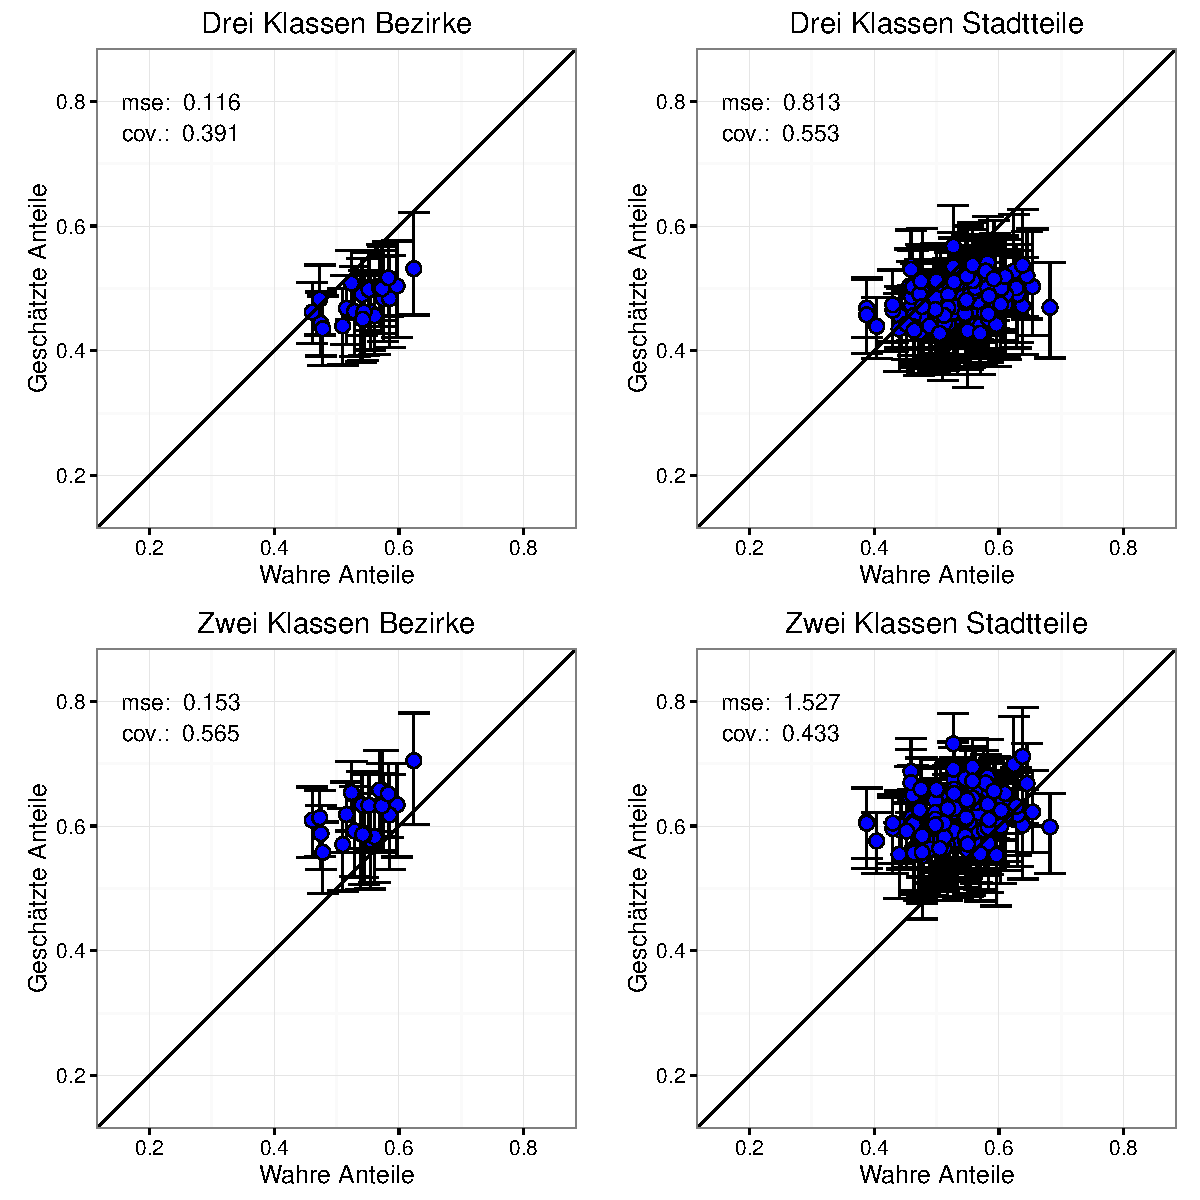
\includegraphics[scale=0.8]{Pictures/PaT}
 \caption{Illustration geschätzte gegen wahre Anteile für Gauss-Krüger Informationen extrapoliert auf die Bürgerumfrage mit zwei und drei Klassenmodell mit 95\% Quantielen}
 \label{vali4}
 \end{center}
\end{figure}

\subsection{Extrapolation}

\begin{figure}[h]
 \begin{center}
 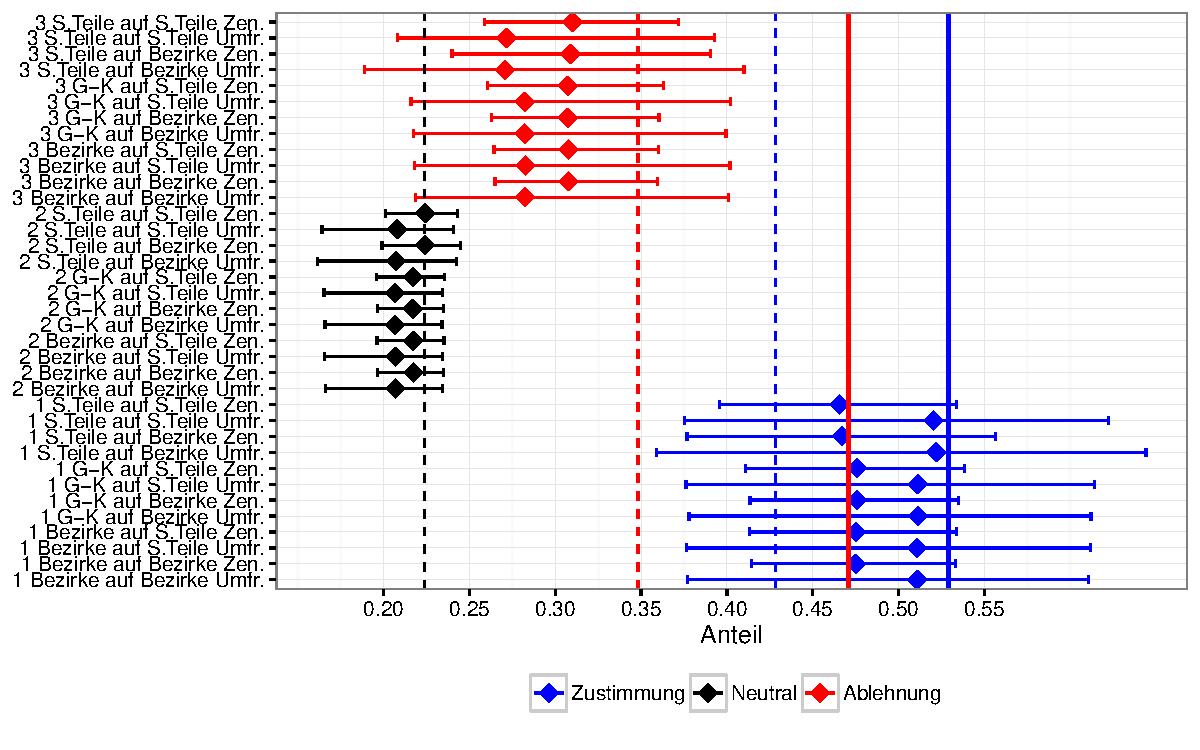
\includegraphics[scale=0.8]{Pictures/S21AlleModelle}
 \caption{Vergleich der extrapolierten Gesamtanteile für Stuttgart mit allen geschätzten Modellen und beiden Extrapolationsdateien mit den wahren Anteilen, sowie den Anteilen der Stichprobe mit 95\% Quantielen zur Meinung zu Stuttgart 21}
 \label{S21Alle}
 \end{center}
\end{figure}


\begin{figure}[h]
 \begin{center}
 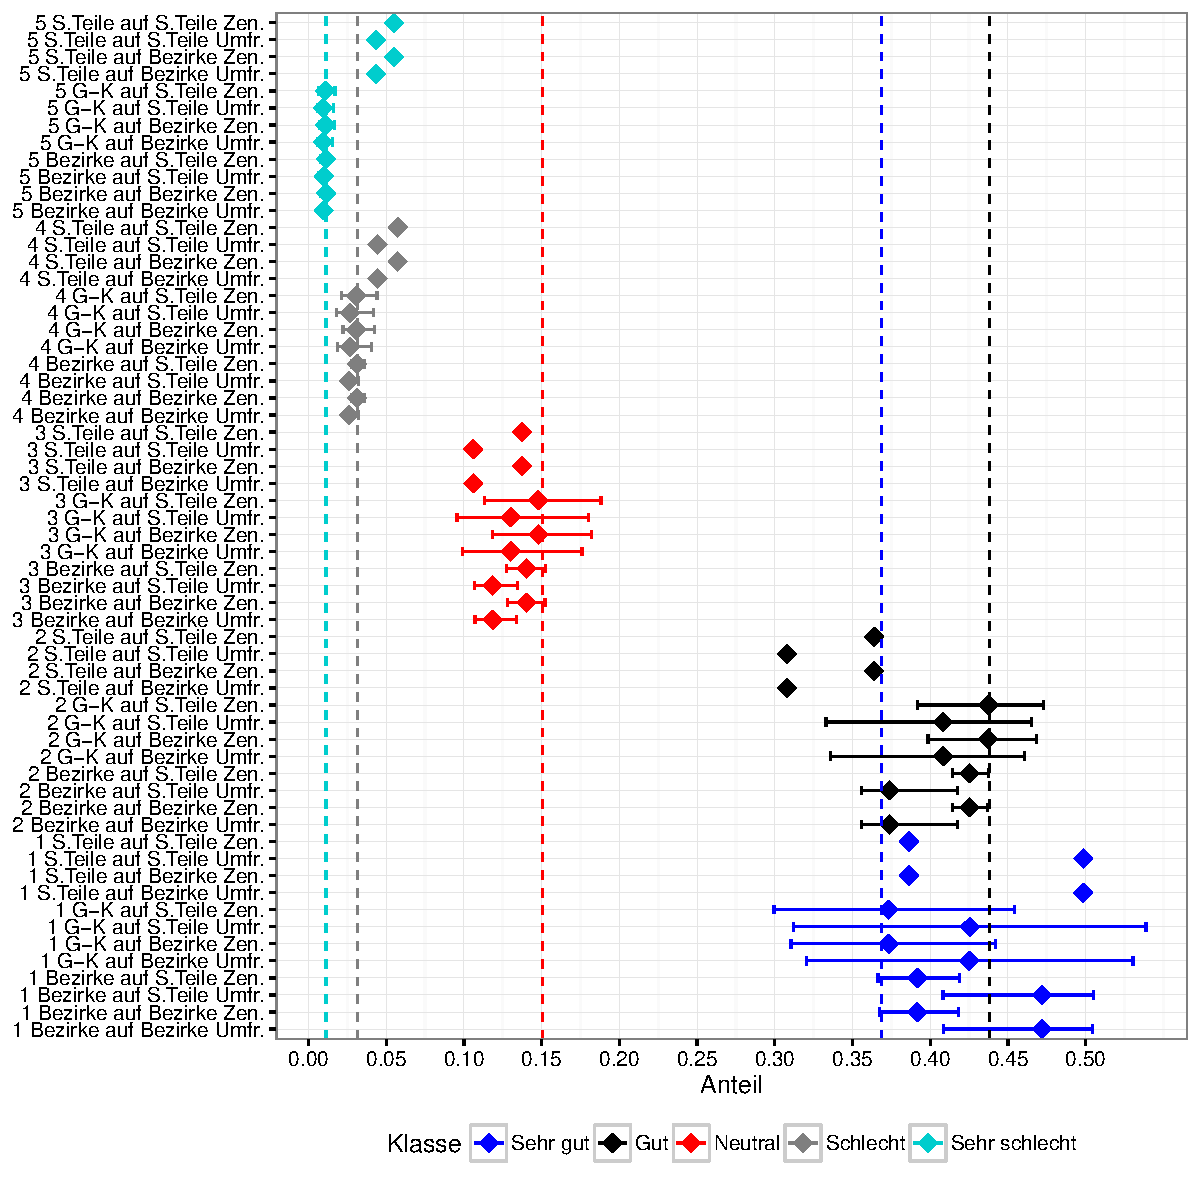
\includegraphics[scale=0.8]{Pictures/WohngegendAlleModelle}
 \caption{Vergleich der extrapolierten Gesamtanteile für Stuttgart mit allen geschätzten Modellen und beiden Extrapolationsdateien mit den Anteilen der Stichprobe mit 95\% Quantielen zur Bewertung der Wohngegend}
 \label{WAlle}
 \end{center}
\end{figure}
%\clearpage

\section{Diskussion}
Die beiden Datensätze zur Grundgesamtheit stammen aus einer Bürgerumfrage mit 470.190 Beobachtungen und dem Zensus mit 380.238 Beobachtungen. Im Verhältnis zu den Grundgesamtheiten dieser Größenordnung sind 3143 Beobachtungen in der Stichprobe relativ gering, was eine gewisse Unsicherheit für die Extrapolation mit sich bringt [...].\\
Weiterhin ist zu beachten, dass Informationen zu dem monatlichen Netto Haushaltseinkommen in beiden Grundgesamtheiten fehlen und somit die Variable nicht für die Prognose verwendet werden kann. Auch war eine denkbare Erstellung von Proxy-Variablen nicht möglich. Eine genaue Auflistung der enthaltenen Variablen aus den Grundgesamtheiten ist im Anhang verfügbar. Die Arbeit zielt darauf ab, die Meinung der Befragten zu dem Projekt Stuttgart 21 und die Zufriedenheit mit der Wohngegend der Befragten auf die Grundgesamtheit zu extrapolieren. Daher ist es sinnvoll die Ausprägungen dieser Variablen genauer zu untersuchen.\\


Insgesamt ist zu sagen, dass die Gauss-Krüger Informationen ein relativ klaren Einblick in die Verteilung der Beobachtungen in der jeweiligen Klasse geben. Bei den diskreten räumlichen Informationen könnte die grobe Aufteilung auf Bezirksebene zu einem Underfitting und die sehr feine Aufteilung auf Stadtteilebene zu einem Overfitting führen [...]. Zudem ist zu vermuten, dass die räumlichen Informationen einen stärkeren Effekt auf die Bewertung der Wohngegend haben, als auf die Meinung zu Stuttgart 21.
%============================================== Conlcusion =========================================================%

\section{Fazit}

\clearpage


%============================================ References ===========================================================%
\addcontentsline{toc}{section}{\numberline{}Literatur}
\bibliographystyle{apalike}
\bibliography{LiteraturStuttgart.bib} 

%\section{References}
%\renewcommand{\section}[2]{}
%\addcontentsline{toc}{section}{References}
%\renewcommand{\bibname}{4 References}
%\phantomsection
%\addcontentsline{toc}{section}{References}




\clearpage

%============================================== Appendix ============================================================%
%\appendix
%\pagestyle{Myheadings}
\chead{ANHANG}
%\pagestyle{}
%\section{$A^{-1}$ Appendix}
%\setcounter{secnumdepth}{0}

\begin{appendix}

\section*{Anhang}
\addcontentsline{toc}{section}{\numberline{}Anhang}






\begin{figure}[h]
 \begin{center}
 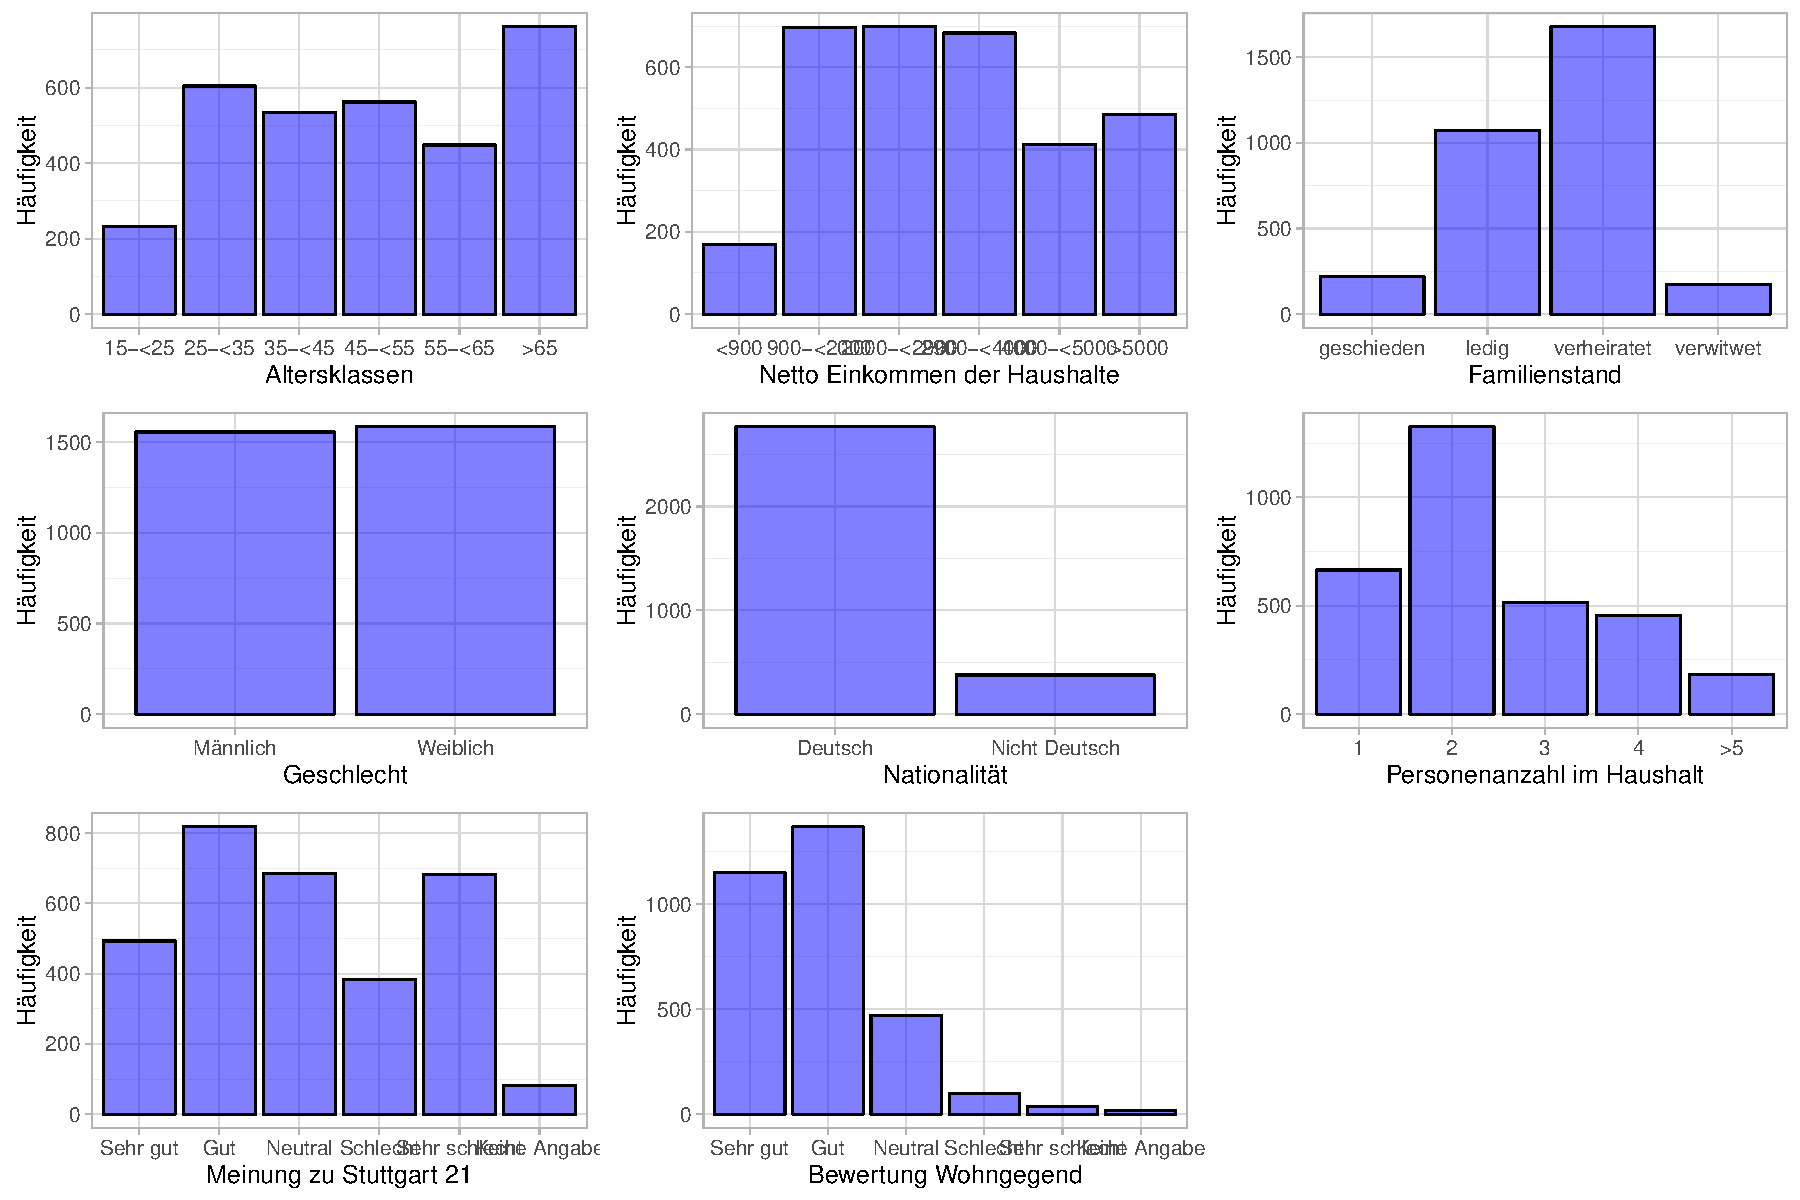
\includegraphics[scale=0.8]{Pictures/BarData}
 \end{center}
\end{figure}


\begin{figure}[h]
 \begin{center}
 
\includegraphics[scale=0.8]{Pictures/BWohn}
 \caption{Anteile der Bewertung der Wohngegend nach Stadtbezirken.}
 \label{BWohn}
 \end{center}
\end{figure}

\begin{figure}[h]
 \begin{center}
 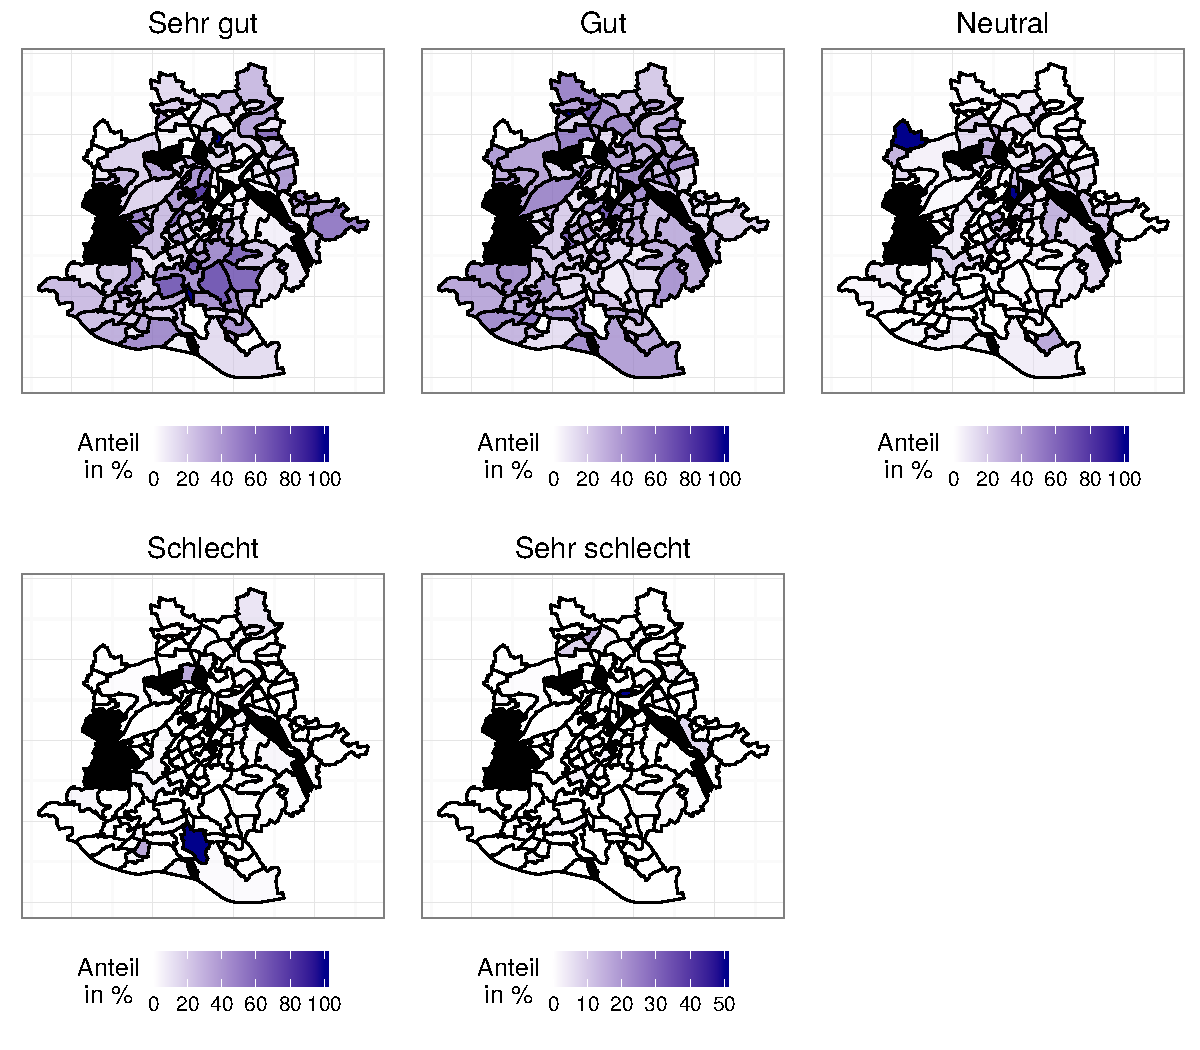
\includegraphics[scale=0.8]{Pictures/SWohn}
 \caption{Anteile der Bewertung der Wohngegend nach Stadtteilen. Wegen der deutlichen unterschiede in den Anteilen sind die Farbskalen nicht einheitlich, sondern unterscheiden sich in den Diagrammen.}
 \label{SWohn}
 \end{center}
\end{figure}

%\begin{figure}[h]
% \begin{center}
% 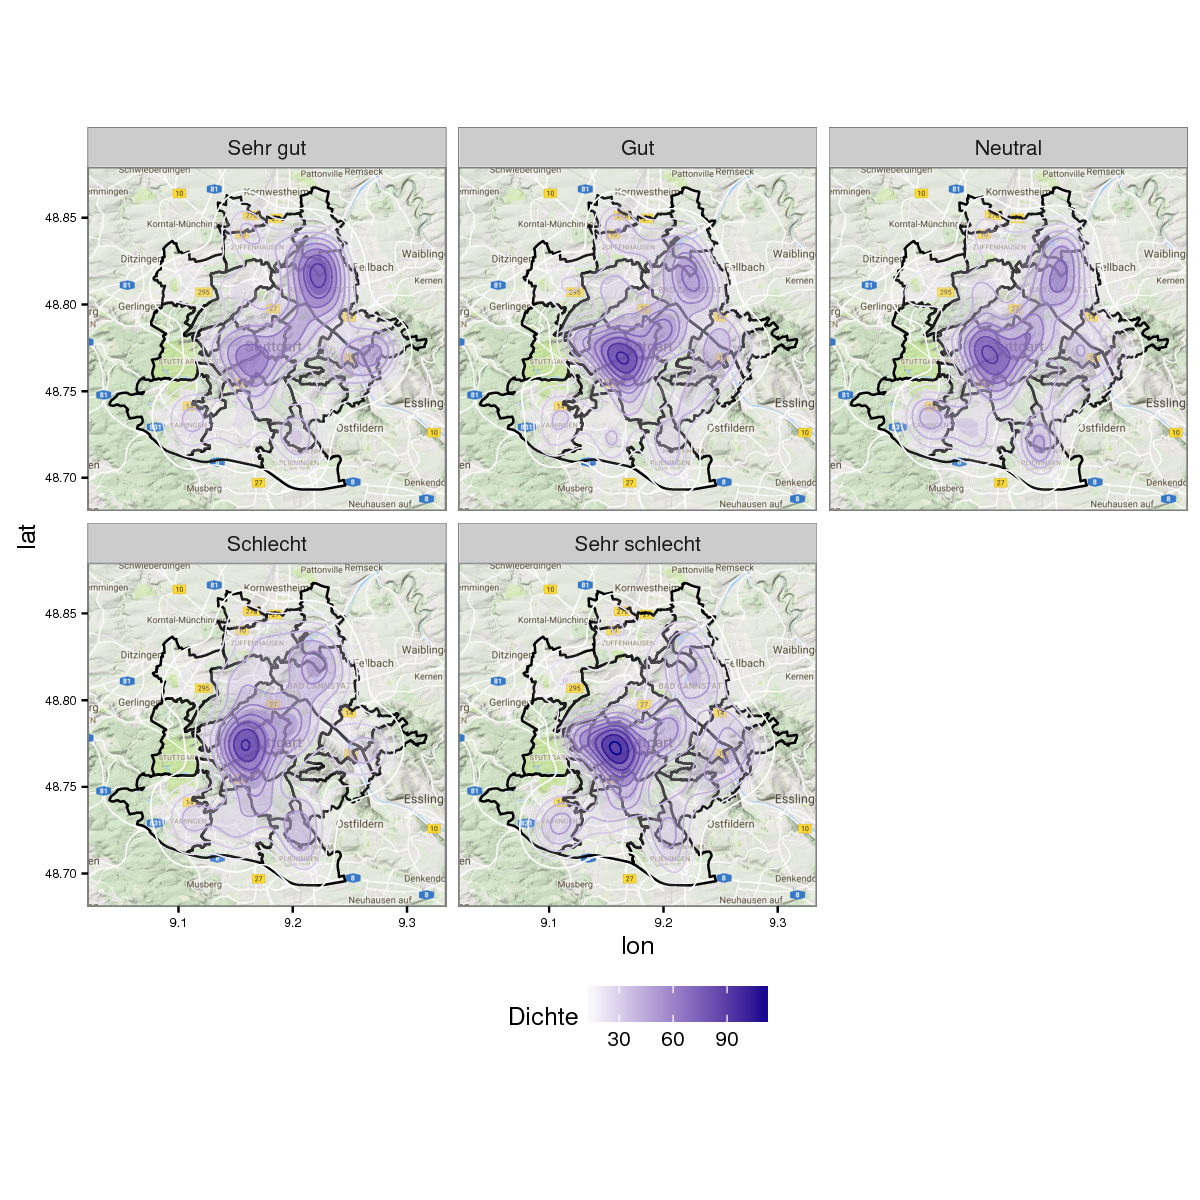
\includegraphics[scale=0.8]{Pictures/XYStuttgart5}
% \caption{Gauss Krüger Informationen Stuttgart 21 (2)}
% \label{endogene}
% \end{center}
%\end{figure}

\end{appendix}
\clearpage
\pagestyle{plain}
%\phantomsection
%\addcontentsline{toc}{section}{Eigenständigkeitserklärung}

%\section{Eigenständigkeitserklärung}

Hiermit versichere ich, dass ich die vorliegende Hausarbeit selbstständig verfasst und keine anderen als die angegebenen
Hilfsmittel benutzt habe. Alle wörtlich oder sinngemäß den Schriften anderer entnommenen Stellen
habe ich unter Angabe der Quellen kenntlich gemacht. Dies gilt auch für beigefügte Zeichnungen, Skizzen, bildliche
Darstellungen und dergleichen.\\
\\
Mir ist bewusst, dass ich mich im Falle einer unbeabsichtigten oder vorsätzlichen Missachtung durch den fehlerhaften
Umgang mit Quellen unter Umständen strafbar mache und die vorliegende Hausarbeit mit nicht ausreichend
bewertet wird.
\\
\\Göttingen, den
\\Unteschrift
\vspace*{4cm}
\\
Hiermit erlaube ich, dass meine Arbeit auf Betrug und falsche, sowie fehlende Zitate auch online geprüft wird.\\
\\
Mir ist bewusst, dass ich mich im Falle einer unbeabsichtigten oder vorsätzlichen Missachtung durch den fehlerhaften
Umgang mit Quellen unter Umständen strafbar mache und die vorliegende Hausarbeit mit nicht ausreichend
bewertet wird.
\\
\\Göttingen, den
\\Unterschrift
\clearpage


\end{document}
